% arara: lualatex: { shell: true, interaction: nonstopmode }
% arara: makeglossaries
% arara: biber
% arara: lualatex: { shell: true, interaction: nonstopmode }
% arara: lualatex: { synctex: true, shell: true, interaction: nonstopmode }

\providecommand{\toplevel}{..}
\providecommand{\sharedPath}{\toplevel/Shared}
\providecommand{\importPath}{\sharedPath/Imports}
\providecommand{\bibPath}{\sharedPath/bibFiles}
\providecommand{\assetPath}{\toplevel/Assets}
\providecommand{\luacodePath}{\toplevel/Shared/luaCode}

% Demo report and presentation prepared by Aaron English (humdrumcomet on github)
\documentclass{beamer}

\usetheme[progressbar=frametitle, numbering=fraction]{metropolis}

\usepackage[mode=build, subpreambles=false]{standalone}
\usepackage{import} % needed for importing with path consideration
\usepackage{geometry} % useful for defining page geometries
\usepackage{hyperref} % used for creating hyperlinks in documents. Both to the web and within the document itself
\makeatletter
\@ifclassloaded{beamer}{
  \typeout{
    -------------------------------------------------
    -------------------------------------------------
    this file is a beamer file, skipping AMS packages
    -------------------------------------------------
    -------------------------------------------------
  }
}{
  \typeout{
    ----------------------------------------------------
    ----------------------------------------------------
    this file is not a beamer file, loading AMS packages
    ----------------------------------------------------
    ----------------------------------------------------
  }
  \usepackage[tbtags]{amsmath} % for typesetting math (American Mathematical Society)
  \usepackage{amsfonts} % fonts and mathematical symbols
  \usepackage{amssymb} % more mathematical symbols
}
\makeatother
% Not needed with lualatex
% \usepackage[utf8]{inputenc} % how to treat the written file (as utf8)
% \usepackage{morewrites} % important because with the glossaries, and beamers own files it is writing out, latex can use up its own hardcoded limit
\usepackage[T1]{fontenc} % the encoding for the output file T1 is the most common, includes accents and many other commonly needed/used characters
\usepackage{hologo}
\usepackage[style=ieee,backend=biber]{biblatex} % for handling bibliographies
\usepackage{float} % added control over
\usepackage{graphicx} % tools for inclusion of graphics
\usepackage{booktabs} % adding commands to improve the look of tables
\usepackage{csvsimple} % simplify table creation by importing .csv files directly
\usepackage{siunitx} % consistent notation and correct formatting of units
\DeclareSIUnit{\torr}{Torr} % Custom unit definition
\usepackage{minted} % inclusion of code blocks with syntax highlighting and
\setminted{linenos, autogobble, fontsize=\footnotesize, breaklines=true} % set global options for minted environments
\usepackage{chemformula} % for writing chemical formulae
\usepackage[useregional]{datetime2}
\usepackage{catchfilebetweentags} % taking elements from between tags

\usepackage[debug, toc, section=section, acronym, symbols]{glossaries} % Glossaries package
\usepackage{tikz}
    \usetikzlibrary{math, arrows, circuits.ee.IEC, positioning, shapes.arrows, shapes.geometric, automata}
\usepackage{pgfplots}
    \pgfplotsset{compat=newest, compat/show suggested version=false}
    \usepgfplotslibrary{groupplots}
\usepackage[siunitx,american voltages, american currents, RPvoltages]{circuitikz}

% A command for less cramped nested fractions
\newcommand\ddfrac[2]{\frac{\displaystyle #1}{\displaystyle #2}}

% Front matter, main matter, and back matter definitions
\def\frontmatter{%
 \pagenumbering{roman}
 \setcounter{page}{1}
 \renewcommand{\thesection}{\roman{section}}
}%
\def\mainmatter{%
 \pagenumbering{arabic}
 \setcounter{page}{1}
 \setcounter{section}{0}
 \renewcommand{\thesection}{\arabic{section}}
}%
\def\backmatter{%
 \setcounter{section}{0}
 \renewcommand{\thesection}{\alph{section}}
}%

%Get rounded wire jumps
\tikzset{
    declare function={% in case of CVS which switches the arguments of atan2
        atan3(\a,\b)=ifthenelse(atan2(0,1)==90, atan2(\a,\b), atan2(\b,\a));},
        kinky cross radius/.initial=+.125cm,
        @kinky cross/.initial=+, kinky crosses/.is choice,
        kinky crosses/left/.style={@kinky cross=-},kinky crosses/right/.style={@kinky cross=+},
        kinky cross/.style args={(#1)--(#2)}{
        to path={
          let \p{@kc@}=($(\tikztotarget)-(\tikztostart)$),
              \n{@kc@}={atan3(\p{@kc@})+180} in
          -- ($(intersection of \tikztostart--{\tikztotarget} and #1--#2)!%
                 \pgfkeysvalueof{/tikz/kinky cross radius}!(\tikztostart)$)
          arc [ radius     =\pgfkeysvalueof{/tikz/kinky cross radius},
                start angle=\n{@kc@},
                delta angle=\pgfkeysvalueof{/tikz/@kinky cross}180 ]
          -- (\tikztotarget)}}
      }

% SI unit pkg conf
\sisetup{
    load-configurations = abbreviations,
    detect-family = true,
    per-mode = reciprocal
}%
\DeclareSIUnit{\torr}{Torr}

% Bibliography .bib file locations should maybe be local?
\addbibresource[location=local]{./accelerators.bib}

% For using the standalone package
\newboolean{standaloneFlag}
\setboolean{standaloneFlag}{true}
% Add Constants list using glossary
\newglossary[cgls]{constants}{cstog}{cstig}{Constants}

% Alphabetize glossary and acronyms list
\makeglossaries


% Command to conditionally typeset a bibliography.
\newcommand{\standaloneBib}{%%
  \ifthenelse{\boolean{standaloneFlag}}%%
  {\printbibliography[heading=bibintoc]
        \printglossary[type=symbols]
        \printglossary[type=acronymtype]
  \printglossary[type=main]}{}}

\DTMsavedate{presentation}{2022-11-19}

%%%%%%%%%%%%%%%%%%%
%%%%%%%%%%%%%%%% Acronym Only
\newglossaryentry{ndfeb}
{
    type=\acronymtype,
    name={NdFeB},
    description={Neodymium Iron Boron Rare Earth Permanent Magnet},
    first={Neodymium iron boron (NdFeB)}
}

%%%%%%%%%%%%%%%%%%%
%%%%%%%%%%%%%%%% Glossary Only
\newglossaryentry{cpp}
{%
    name={C++},
    description={C++ is a programming language that can be used as an object oriented programming language, an imperative programming language, and still provide low-level memory control. Note: All C++ code used in this work is compiled under the C++11 standard}
}
%%%%%%%%%%%%%%%%%%%
%%%%%%%%%%%%%%%% Glossary and Acronym
% Self referencing glossary entry to minimize what needs to be edited between changes
\newglossaryentry{cwvmg}
{
    name={\glsentrytext{cwvm}},
    description={\glsentrydesc{cwvm} (\glsentrytext{cwvm}) is a voltage multiplier that can be cascaded to give an output voltage of \(nV_{p-p}\) with \(n\) being the number of stages}
}
\newglossaryentry{cwvm}
{
    type=\acronymtype,
    name={CWVM},
    description={Cockroft-Walton voltage multiplier},
    first={\glsentrydesc{cwvm} (\glsentrytext{cwvm})\glsadd{cwvmg}},
    plural={\glsentrytext{cwvm}s},
    descriptionplural={\glsentrydesc{cwvm}s},
    firstplural={\glsentrydescplural{cwvm} (\glsentryplural{cwvm})},
    see=[Glossary:]{cwvmg}
}


\luastringsubs{
  {Acorn-RiscPC-LaTeX.pdf}={\assetPath/Images/InkscapeDemo/Acorn-RiscPC-LaTeX.pdf},
  {Risc PC system organisation}={\textbf{\huge Risc \glstext{pc} system organisation}},
  {ARMCPU}={{\textbf{\Large ARM \glstext{cpu}}}},
  {2nd CPU}={\textbf{\Large 2\textsuperscript{nd} \glstext{cpu}}},
  {VRAM}={\textbf{\Large\glstext{vram}}},
  {DRAM}={\textbf{\Large \glstext{dram}}},
  {i/f ASIC}={\textbf{\Large \glstext{i/f} \glstext{asic}}},
  {expansion cards}={\textbf{\Large expansion cards}},
  {IDE disk}={\textbf{\Large \glstext{ide} disk}},
  {floppy disc}={\textbf{\Large floppy disc}},
  {ROM}={\textbf{\Large \glstext{rom}}},
  {RTC}={\textbf{\Large \glstext{rtc}}},
  {I2C}={\textbf{\Large \glstext{i2c}}},
  {IOMD}={\textbf{\Large \glstext{iomd}}},
  {network}={\textbf{\Large network}},
  {UPC}={\textbf{\Large \glstext{upc}}},
  {parallel i/f}={\textbf{parallel \glstext{i/f}}},
  {serial i/f}={\textbf{serial \glstext{i/f}}},
  {Lo 16-bit buffered I/O data}={\textbf{Lo \SI{16}{b} buffered \glstext{i/o} data}},
  {video}={\textbf{\large video}},
  {VIDC20}={\textbf{\Large VIDC20}},
  {data bus}={\textbf{\large data bus}},
  {mux addr}={\textbf{\large \glstext{mux} addr.}},
  {address bus}={\textbf{\large address bus}},
  {serial\\data}={\textbf{\large serial}\\ \textbf{\large data }},
  {analogue\\sound}={\textbf{\large analogue}\\ \textbf{\large sound}},
  {latched\\address\\bus}={\textbf{\large latched}\\ \textbf{\large address} \\ \textbf{\large bus}},
  {Hi 16-bit\\I/O data}={\textbf{\large Hi \SI{16}{b}}\\ \textbf{\large \glstext{i/o} data}},
}{\assetPath/Images/InkscapeDemo/Acorn-RiscPC-LaTeX.pdf_tex}{\assetPath/Images/InkscapeDemo/Acorn-RiscPC-LaTeX-subbed-pdf-tex.tex}

\luastringsubs{
  {Acorn-RiscPC-LaTeX.pdf}={\assetPath/Images/InkscapeDemo/Acorn-RiscPC-LaTeX.pdf},

}{\assetPath/Images/InkscapeDemo/Acorn-RiscPC-LaTeX.pdf_tex}{\assetPath/Images/InkscapeDemo/Acorn-RiscPC-LaTeX-subbed-path.tex}


\title{\LaTeX~in Different Environments}
\author{Ghassan Arnouk \and
            Alec Bales D'Cruze \and
            Aaron English}

\begin{document}
    \begin{frame}
        \titlepage
    \end{frame}
    \begin{frame}[noframenumbering, plain]
        \frametitle{Contents}
        \tableofcontents
    \end{frame}
    \section{The \TeX~Family Tree}
        \begin{frame}
            \frametitle{The Most Common Members}
            \includestandalone[mode=tex, width=\textwidth]{\assetPath/Images/Tikz/texfamilytree/texfamilytree}
        \end{frame}
    \section{Processing \TeX~Files}
        \begin{frame}[t,fragile]
            \frametitle<-5>{The \TeX~Procedure}
                \includestandalone[mode=tex, height=0.3\textheight]{\assetPath/Images/Tikz/texFlow/texFlow}
                \begin{onlyenv}<2>
                    \begin{table}
                        \centering
                        \caption{\LaTeX~Specific Editors}
                        \begin{tabular}{cccc}
                            & Linux & MacOS & Windows \\
                            TeXStudio & \checkmark & \checkmark & \checkmark \\
                            TeXMaker  & \checkmark & \checkmark & \checkmark \\
                            TeXnicCenter  & \checkmark & \checkmark & \checkmark \\
                        \end{tabular}
                    \end{table}
                \end{onlyenv}
                \begin{onlyenv}<3>
                    \begin{table}
                        \centering
                        \caption{Generic Text Editors with \LaTeX~Specific Extra's}
                        \begin{tabular}{cccc}
                            & Linux & MacOS & Windows \\
                            Emacs & \checkmark & \checkmark & \checkmark \\
                            Vim  & \checkmark & \checkmark & \checkmark \\
                            VSCode  & \checkmark & \checkmark & \checkmark \\
                            Sublime Text & \checkmark & \checkmark & \checkmark
                        \end{tabular}
                    \end{table}
                \end{onlyenv}
                \begin{onlyenv}<4>
                    \begin{table}
                        \centering
                        \caption{\TeX~Distributions for Different Operating Systems}
                        \centering
                        \begin{tabular}{cccc}
                            & Linux & MacOS & Windows \\
                            TeXLive & \checkmark & \checkmark & \checkmark \\
                            MacTeX  &  & \checkmark &  \\
                            MiKTeX  &  &  & \checkmark \\
                            ProTeXt &  &  & \checkmark
                        \end{tabular}
                    \end{table}
                \end{onlyenv}
                \frametitle<5>{Manually in Shell/Bash/Etc.}
                \begin{onlyenv}<5>
                    \begin{centering}
                        \begin{minted}{bash}
                            pdflatex --shell-escape --interaction=nonstopmode report
                            biber report
                            makeglossaries report
                            pdflatex --shell-escape --interaction=nonstopmode report
                            pdflatex --shell-escape --interaction=nonstopmode report
                        \end{minted}
                    \end{centering}
                \end{onlyenv}
                \frametitle<6>{Passing Commands at Compile Time}
                \begin{onlyenv}<6>
                    \begin{centering}
                        \begin{minted}{bash}
                            lualatex --shell-escape --interaction=nonstopmode "\\providecommand{\\iswhichmode}{draft} \\input{report}"
                            biber report
                            makeglossaries report
                            lualatex --shell-escape --interaction=nonstopmode "\\providecommand{\\iswhichmode}{draft} \\input{report}"
                            lualatex --shell-escape --interaction=nonstopmode "\\providecommand{\\iswhichmode}{final} \\input{report}"
                        \end{minted}
                    \end{centering}
                \end{onlyenv}
                \frametitle<7>{latexmk}
                \begin{onlyenv}<7>
                    \begin{centering}
                        \begin{minted}{bash}
                            latexmk -pdf report.tex
                        \end{minted}
                    \end{centering}
                \end{onlyenv}
                \frametitle<8>{ARARA}
                \begin{onlyenv}<8>
                    \begin{centering}
                        \begin{minted}{latex}
                            % arara: lualatex: { shell: true, interaction: nonstopmode }
                            % arara: makeglossaries
                            % arara: biber
                            % arara: lualatex: { shell: true, interaction: nonstopmode }
                            % arara: lualatex: { synctex: true, shell: true, interaction: nonstopmode }
                        \end{minted}
                        \begin{minted}{bash}
                            arara -v report.tex
                        \end{minted}
                    \end{centering}
                \end{onlyenv}
        \end{frame}
    \section{External Tools}
        \begin{frame}[t,fragile]
            \frametitle{Matplotlib - Python Plotting}
            \begin{columns}[onlytextwidth]
                \begin{column}[T]{0.75\textwidth}
                    \begin{onlyenv}<1>
                        \inputminted{python}{\assetPath/Code/matplotlibexample.py}
                    \end{onlyenv}
                    \begin{onlyenv}<2>
                        \inputminted[firstline=29,lastline=45]{latex}{\assetPath/Code/examplePlot.tex}
                    \end{onlyenv}
                    \begin{onlyenv}<3>
                        \begin{minted}{latex}
                        \begin{figure}[H]
                        \begin{centering}
                        \includegraphics[width=0.5\textwidth] {\assetPath/Code/examplePlot.tex}
                        \caption{A figure produced with matplotlib}
                        \label{fig:test}
                        \end{centering}
                        \end{figure}
                        \end{minted}
                    \end{onlyenv}
                    \only<4>{\includestandalone[mode=tex, width=\textwidth]{\assetPath/Code/examplePlot}}
                \end{column}\hfill
                \begin{column}[T]{0.2\textwidth}
                    \centering
                    \includestandalone[mode=tex, width=\textwidth]{\assetPath/Images/Tikz/matplotlibFlow/matplotlibflow}
                \end{column}
            \end{columns}
        \end{frame}
        \begin{frame}[t,fragile]
            \frametitle{Sympy - Symbolic Math in Python}
            \begin{columns}[onlytextwidth]
                \begin{column}[T]{0.75\textwidth}
                    \begin{onlyenv}<1>
                        \inputminted{python}{\assetPath/Code/sympyexample.py}
                    \end{onlyenv}
                    \begin{onlyenv}<2>
                        \begin{minted}{latex}
                        \begin{equation}a^{b} e + \frac{c}{d}\end{equation}
                        \begin{equation}\frac{\partial}{\partial b} \left(a^{b} e + \frac{c}{d}\right) = a^{b} e \log{\left(a \right)}\end{equation}
                        \begin{equation}\int \left(a^{b} e + \frac{c}{d}\right)\, da = \frac{a c}{d} + \frac{a^{b + 1} e}{b + 1}\end{equation}
                        \end{minted}
                    \end{onlyenv}
                    \only<3>{
                        \begin{equation}a^{b} e + \frac{c}{d}\end{equation}
                        \begin{equation}\frac{\partial}{\partial b} \left(a^{b} e + \frac{c}{d}\right) = a^{b} e \log{\left(a \right)}\end{equation}
                        \begin{equation}\int \left(a^{b} e + \frac{c}{d}\right)\, da = \frac{a c}{d} + \frac{a^{b + 1} e}{b + 1}\end{equation}
                    }
                \end{column}\hfill
                \begin{column}[T]{0.2\textwidth}
                    \centering
                    \includestandalone[mode=tex, width=\textwidth]{\assetPath/Images/Tikz/sympyFlow/sympyflow}
                \end{column}
            \end{columns}
        \end{frame}
        \begin{frame}[t,fragile]
            \frametitle{Inkscape - Drawing and Manipulating Vector Graphics}
            \begin{columns}[onlytextwidth]
                \begin{column}[T]{0.75\textwidth}
                    \only<1>{
                        \begin{figure}
                        \centering
                        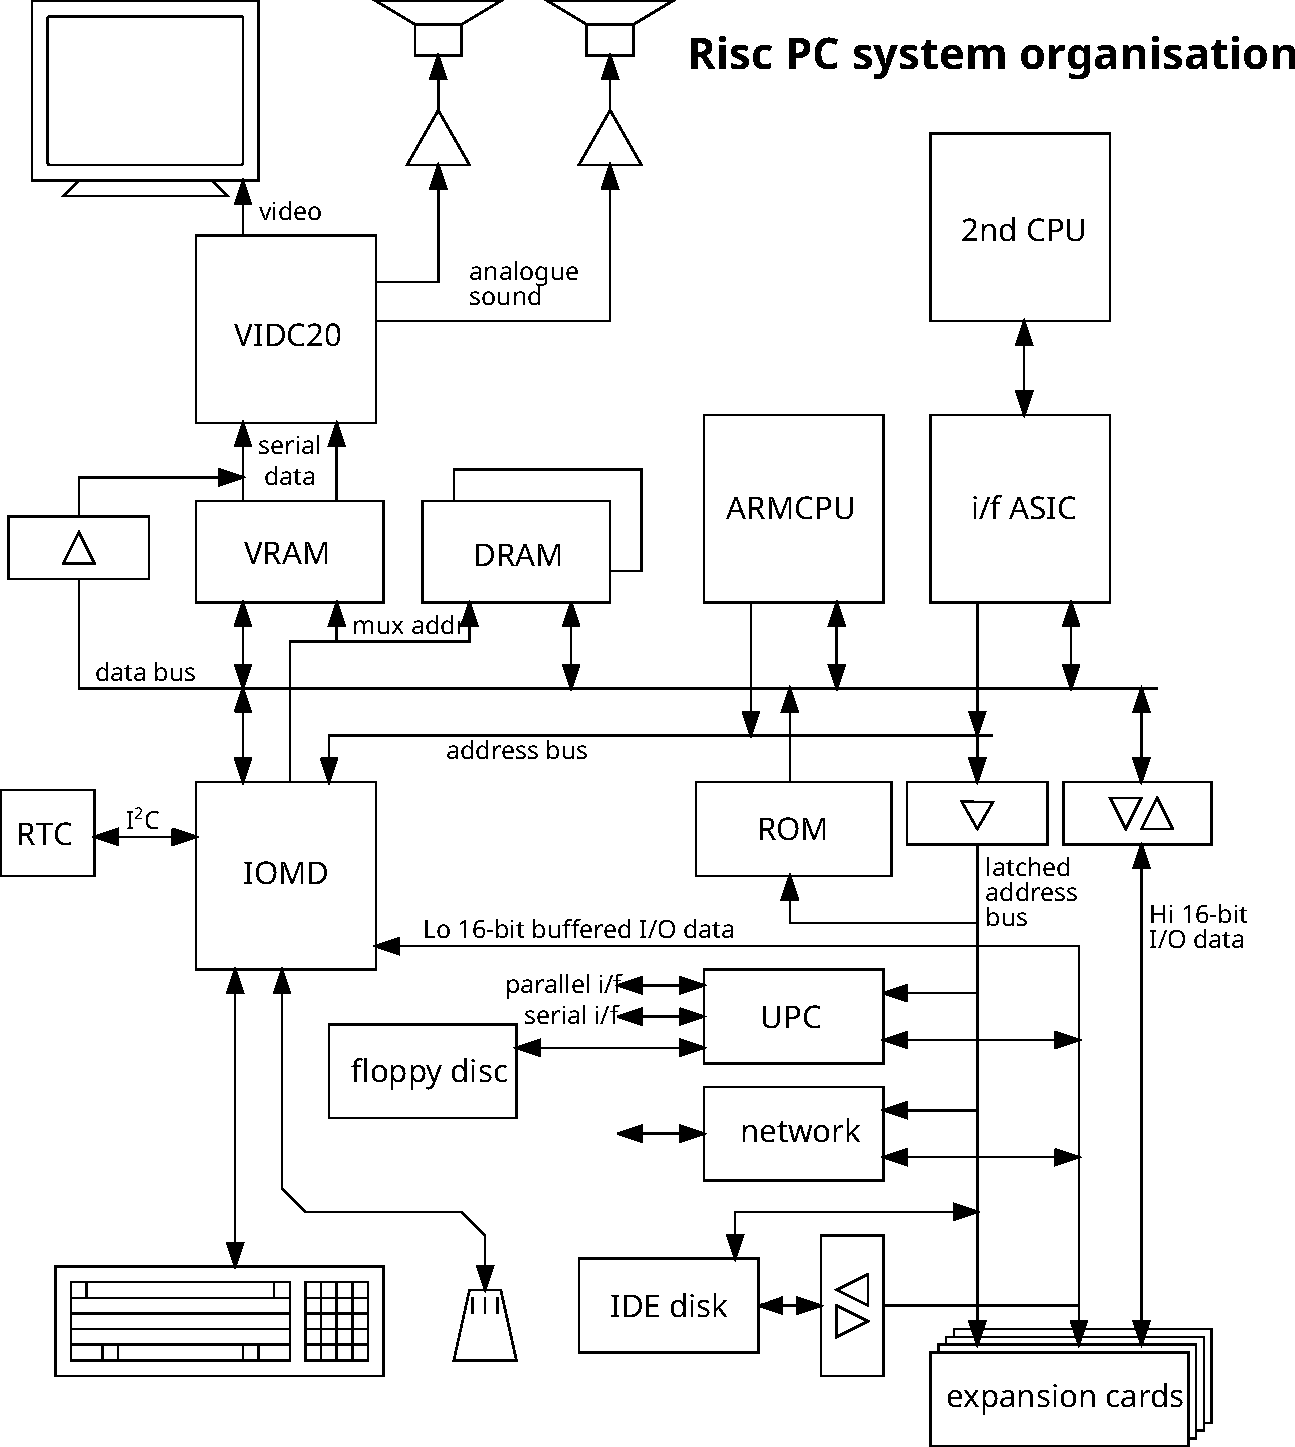
\includegraphics[height=0.7\textheight]{\assetPath/Images/InkscapeDemo/Acorn-RiscPC-PDF-Original}
                        \caption{Original vector graphic block diagram of the Acorn Risc PC \cite{ref:01}}
                        \label{fig:texsub}
                        \end{figure}
                    }
                    \begin{onlyenv}<2>
                        \includestandalone[mode=tex, width=0.9\textwidth]{\assetPath/Images/Tikz/inkscapeConversion/inkscapeConversion}
                    \end{onlyenv}
                    \begin{onlyenv}<3>
                        \inputminted[firstline=27,lastline=46]{latex}{\assetPath/Images/InkscapeDemo/Acorn-RiscPC-LaTeX.pdf_tex}
                    \end{onlyenv}
                    \begin{onlyenv}<4>
                        \begin{minted}{latex}
                        \begin{figure}[H]
                        \begin{centering}
                        \includestandalone[mode=tex, height=0.7\textheight]{\assetPath/Images/InkscapeDemo/Acorn-RiscPC-LaTeX-subbed-path}
                        \caption{Inkscape PDF+\TeX}
                        \label{fig:test}
                        \end{centering}
                        \end{figure}
                        \end{minted}
                    \end{onlyenv}
                    \only<5>{
                        \begin{figure}
                        \centering
                        \includestandalone[mode=tex, height=0.7\textheight]{\assetPath/Images/InkscapeDemo/Acorn-RiscPC-LaTeX-subbed-path}
                        \caption{Directly incorporating Inkscape PDF+\TeX~export of the Acorn Risc PC block diagram}
                        \label{fig:texsub}
                        \end{figure}
                    }
                    \only<6>{
                        \begin{figure}
                        \centering
                        \includestandalone[mode=tex, height=0.7\textheight]{\assetPath/Images/InkscapeDemo/Acorn-RiscPC-LaTeX-subbed-pdf-tex}
                        \caption{Inkscape PDF+\TeX~of the Acorn Risc PC block diagram with substitution of text via \hologo{LuaLaTeX}}
                        \label{fig:texsub}
                        \end{figure}
                    }
                \end{column}\hfill
                \begin{column}[T]{0.2\textwidth}
                    \centering
                    \includestandalone[mode=tex, width=\textwidth]{\assetPath/Images/Tikz/inkscapeFlow/inkscapeflow}
                \end{column}
            \end{columns}
        \end{frame}
    \section{Backmatter}
        \begin{frame}[allowframebreaks]
            \frametitle{Bibliography}
            \printbibliography
        \end{frame}
        \begin{frame}[allowframebreaks]
            \frametitle{Acronyms}
            \printglossary[type=\acronymtype]
        \end{frame}
        % \begin{frame}[allowframebreaks]
        %     \frametitle{Glossary}
        %     \printglossary[type=main]
        % \end{frame}
        % \begin{frame}[allowframebreaks]
        %     \frametitle{Constants}
        %     \printglossary[type=constants, nonumberlist, nopostdot]
        % \end{frame}
        % \begin{frame}[allowframebreaks]
        %     \frametitle{Symbols}
        %     \printglossary[type=symbols]
        % \end{frame}
\end{document}
